\header[hs]{
    \headtitle{L'artilleur de Metz} \label{l-artilleur-de-metz}
    %
    
    \insertComment{Tirée d'un chant millitaire faisant référence aux années messines de l’Ecole d’artillerie (1802-1870).}{}
    %Il existe des versions non paillardes.
}

\textbf{Refrain :}
\enluminure{3}{\href{https://www.youtube.com/watch?v=vPyXuK2r91E}{A}}{rtilleurs}, mes chers frères
\\A sa santé buvons un verre
\\Et répétons ce gai refrain
\\Viv' les artilleurs, les femmes et le bon vin 
\\Et répétons ~~~\bissimple
\\Ce gai refrain \bissimple
\\Viv' les artilleurs, les femmes et le bon vin
\dualcol{
Quand l'artilleur de Metz
\\Arrive en garnison
\\Toutes les femmes de Metz
\\Se foutent le doigt dans l'con
\\Pour préparer l'chemin
\\A l'artilleur rupin
\\Qui leur foutra demain
\\Sa pine dans le vagin
\\\\Quand l'artilleur de Metz
\\Demande une faveur
\\Toutes les femmes de Metz
\\L'accordent avec ardeur
\\Et le mari cornard
\\Voit l'artilleur chicard
\\Baiser également
\\La fille et la maman
\\\\Quand l'artilleur de Metz
\\Quitte sa garnison
\\Toutes les femmes de Metz
\\Se foutent à leur balcon
\\Pour saluer le départ
\\Cet artilleur chicard
\\Qui leur a tant foutu
\\Sa pine au trou du cul

\begin{center}
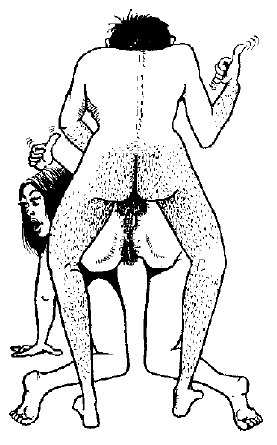
\includegraphics[width=0.4\textwidth]{images/image3.png}
\end{center}

}


\breakpage